\documentclass{article}
\usepackage{graphicx}
\usepackage{hyperref}
\usepackage[T1]{fontenc}
\usepackage{tgadventor}

% Set the font family to sans-serif
\renewcommand{\familydefault}{\sfdefault}

\graphicspath{ {images/} }

\title{Intro Latex}
\author{Owen Gombas}
\date{October 2021}

\begin{document}
\maketitle
\tableofcontents

\section{Introduction}

My first \LaTeX{} document.

% This is a comment

\textbf{Bold text}

\underline{Underline}

\textit{Italic text}

\textbf{My text \emph{emph} is cool}

\textit{My text \emph{emph} is cool}

My text \emph{emph} is cool

\section{Image}
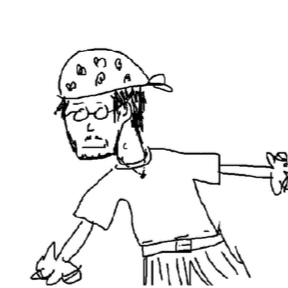
\includegraphics{ven.png}

\section{Lists}
Here is a list
\begin{itemize}
  \item Item 1
  \item Item 2
\end{itemize}

Here is a numerated list
\begin{enumerate}
  \item Item 1
  \item Item 2
\end{enumerate}

\section{Formulas}
\[
  E^{i_1 i_2 \dots i_n}_{j_1 j_2 \dots j_n}
  = T(x^{i_1}, \dots x^{i_2}, \dots, x^{i_n})
\]

\section{Sections}
\begin{abstract}
  This is an abstract
\end{abstract}

\section{Section}
\subsection{Sub section}
\subsubsection{Sub sub section}

\section{Tables}
% c for center, l for left, r for right -centering
\begin{tabular}{ c c c }
  cell1 & cell2 & cell3 \\
  cell1 & cell2 & cell3 \\
  cell1 & cell2 & cell3 \\
\end{tabular}

% c for center, l for left, r for right -centering
\begin{tabular}{ | c | c | c | }
  \hline
  cell1 & cell2 & cell3 \\
  cell1 & cell2 & cell3 \\
  cell1 & cell2 & cell3 \\
  \hline
\end{tabular}

\section{Urls}
\url{https://fr.overleaf.com/learn/latex/Hyperlinks} \\
\href{https://fr.overleaf.com/learn/latex/Hyperlinks}{Named link} \\
\href{http://www.personal.ceu.hu/tex/breaking.htm}{Page break} \\
\href{https://fr.overleaf.com/learn/latex/List_of_Greek_letters_and_math_symbols}{Math symbols}

\end{document}
